\documentclass[8pt,a4paper,compress,handout]{beamer}

\usepackage{/home/siyer/lib/slides}

\title{Translating JVM Code to MIPS Code}
\date{}

\begin{document}
\begin{frame}
\vfill
\titlepage
\end{frame}

\begin{frame}
\frametitle{Outline}
\tableofcontents
\end{frame}

\section{Introduction}
\begin{frame}[fragile]
\pause

Compilation is not necessarily done after the class file is constructed

\pause
\bigskip

At ``execution'', the class is loaded into the JVM and then interpreted

\pause
\bigskip

In the Oracle HotSpot VM, once a method has been executed several times, it is compiled to native code --- code that can be directly executed by the underlying computer

\pause
\bigskip

So at run time, control shifts back and forth between JVM code and native code

\pause
\bigskip

The native code runs much faster than does the interpreted JVM code

\pause
\bigskip

Compiling JVM code to native code involves the following
\begin{itemize}
\item Register allocation
\item Optimization
\item Instruction selection
\item Run-time support
\end{itemize}
\end{frame}

\begin{frame}[fragile]
\pause

We will translate a small subset of JVM instructions to the native code for the MIPS architecture, and execute the native code using SPIM (a MIPS simulator)

\pause
\bigskip

MIPS is a relatively modern reduced instruction set computer (RISC), which has a set of simple but fast instructions that operate on values in registers --- for this reason it is often referred to as a register-based architecture

\pause
\bigskip

Our goal is illustrated in the following figure
\begin{center}
\visible<4->{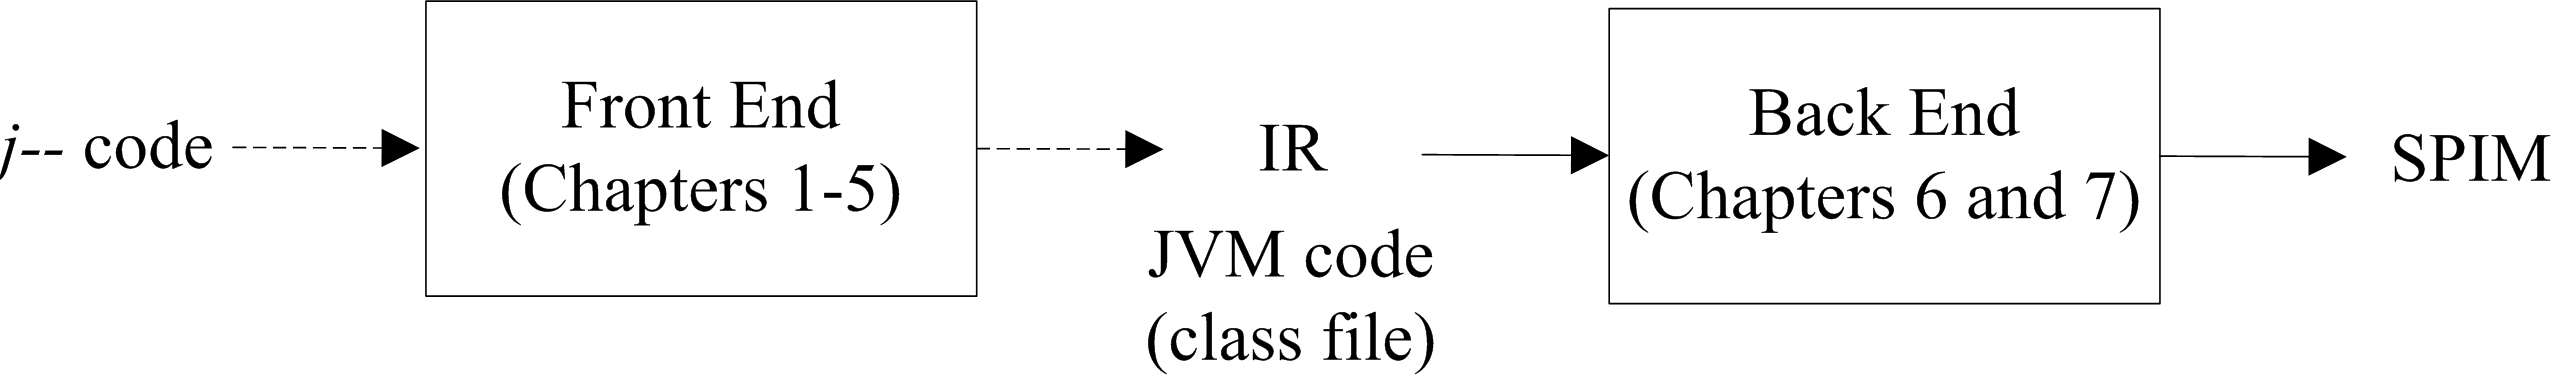
\includegraphics[scale=0.6]{{figures/figure06.01}.jpg}}
\end{center}

We re-define what constitute the IR, the front end and the back end
\begin{itemize}
\item JVM code is our new IR
\item The \jmm to JVM translator (Chapters 1 --- 5) is our new front end
\item The JVM to SPIM translator (Chapters 6 and 7) is our new back end
\end{itemize}

\pause
\bigskip

We translate enough JVM code to SPIM code to handle the \jmm program shown in the following slide
\end{frame}

\begin{frame}[fragile]
\pause

\begin{lstlisting}[language=Java]
import spim.SPIM;

// Prints factorial of a number computed using recursive and iterative
// algorithms.
public class Factorial {
    // Return the factorial of the given number computed recursively.
    public static int computeRec(int n) {
        if (n <= 0) {
            return 1;
        } else {
            return n * computeRec(n - 1);
        }
    }

    // Return the factorial of the given number computed iteratively.
    public static int computeIter(int n) {
        int result = 1;
        while ( n > 0 ) {
            result = result * n--;
	}
        return result;
    }

    // Entry point; print factorial of a number computed using
    // recursive and iterative algorithms.
    public static void main(String[] args) {
        int n = 7;
        SPIM.printInt(Factorial.computeRec(n));
	SPIM.printChar('\n');
        SPIM.printInt(Factorial.computeIter(n));
        SPIM.printChar('\n');
    }
}
\end{lstlisting}
\end{frame}

\begin{frame}[fragile]
\pause

We handle static methods, conditional statements, while loops, recursive method invocations, and enough arithmetic to do a few computations

\pause
\bigskip

We must deal with some objects, for example, constant strings

\pause
\bigskip

The program above refers to an array, but doesn't do anything with it so we do not implement array objects

\pause
\bigskip

So, our run-time support is minimal

\pause
\bigskip

To determine what JVM instructions must be handled, it is worth looking at the output from running \lstinline{javap} on \lstinline{Factorial.class}

\pause
\bigskip

\begin{lstlisting}[language={}]
public class Factorial extends java.lang.Object
  minor version: 0
  major version: 49
  Constant pool:
... <the constant pool is elided here> ...

{
public Factorial();
  Code:
   Stack=1, Locals=1, Args_size=1
   0: aload_0
   1: invokespecial #8; //Method java/lang/Object."<init>":()V
   4: return
\end{lstlisting}
\end{frame}

\begin{frame}[fragile]
\pause

\begin{lstlisting}[language={}]

public static int computeRec(int);
  Code:
   Stack=3, Locals=1, Args_size=1
   0: iload_0
   1: iconst_0
   2: if_icmpgt 10
   5: iconst_1
   6: ireturn
   7: goto  19
   10: iload_0
   11: iload_0
   12: iconst_1
   13: isub
   14: invokestatic #13; //Method computeRec:(I)I
   17: imul
   18: ireturn
   19: nop

public static int computeIter(int);
  Code:
   Stack=2, Locals=2, Args_size=1
   0: iconst_1
   1: istore_1
   2: iload_0
   3: iconst_0
   4: if_icmple 17
   7: iload_1
   8: iload_0
   9: iinc  0, -1
   12: imul
   13: istore_1
   14: goto 2
   17: iload_1
   18: ireturn
\end{lstlisting}
\end{frame}

\begin{frame}[fragile]
\pause

\begin{lstlisting}[language={}]

public static void main(java.lang.String[]);
  Code:
   Stack=1, Locals=2, Args_size=1
   0: bipush    7
   2: istore_1
   3: iload_1
   4: invokestatic  #13; //Method computeRec:(I)I
   7: invokestatic  #22; //Method spim/SPIM.printInt:(I)V
   10: bipush   10
   12: invokestatic #26; //Method spim/SPIM.printChar:(C)V
   15: iload_1
   16: invokestatic #28; //Method computeIter:(I)I
   19: invokestatic #22; //Method spim/SPIM.printInt:(I)V
   22: bipush   10
   24: invokestatic #26; //Method spim/SPIM.printChar:(C)V
   27: return
}
\end{lstlisting}
\end{frame}

\section{SPIM and the MIPS Architecture}
\begin{frame}[fragile]
\pause

The MIPS computer organization is shown below
\begin{center}
\visible<2->{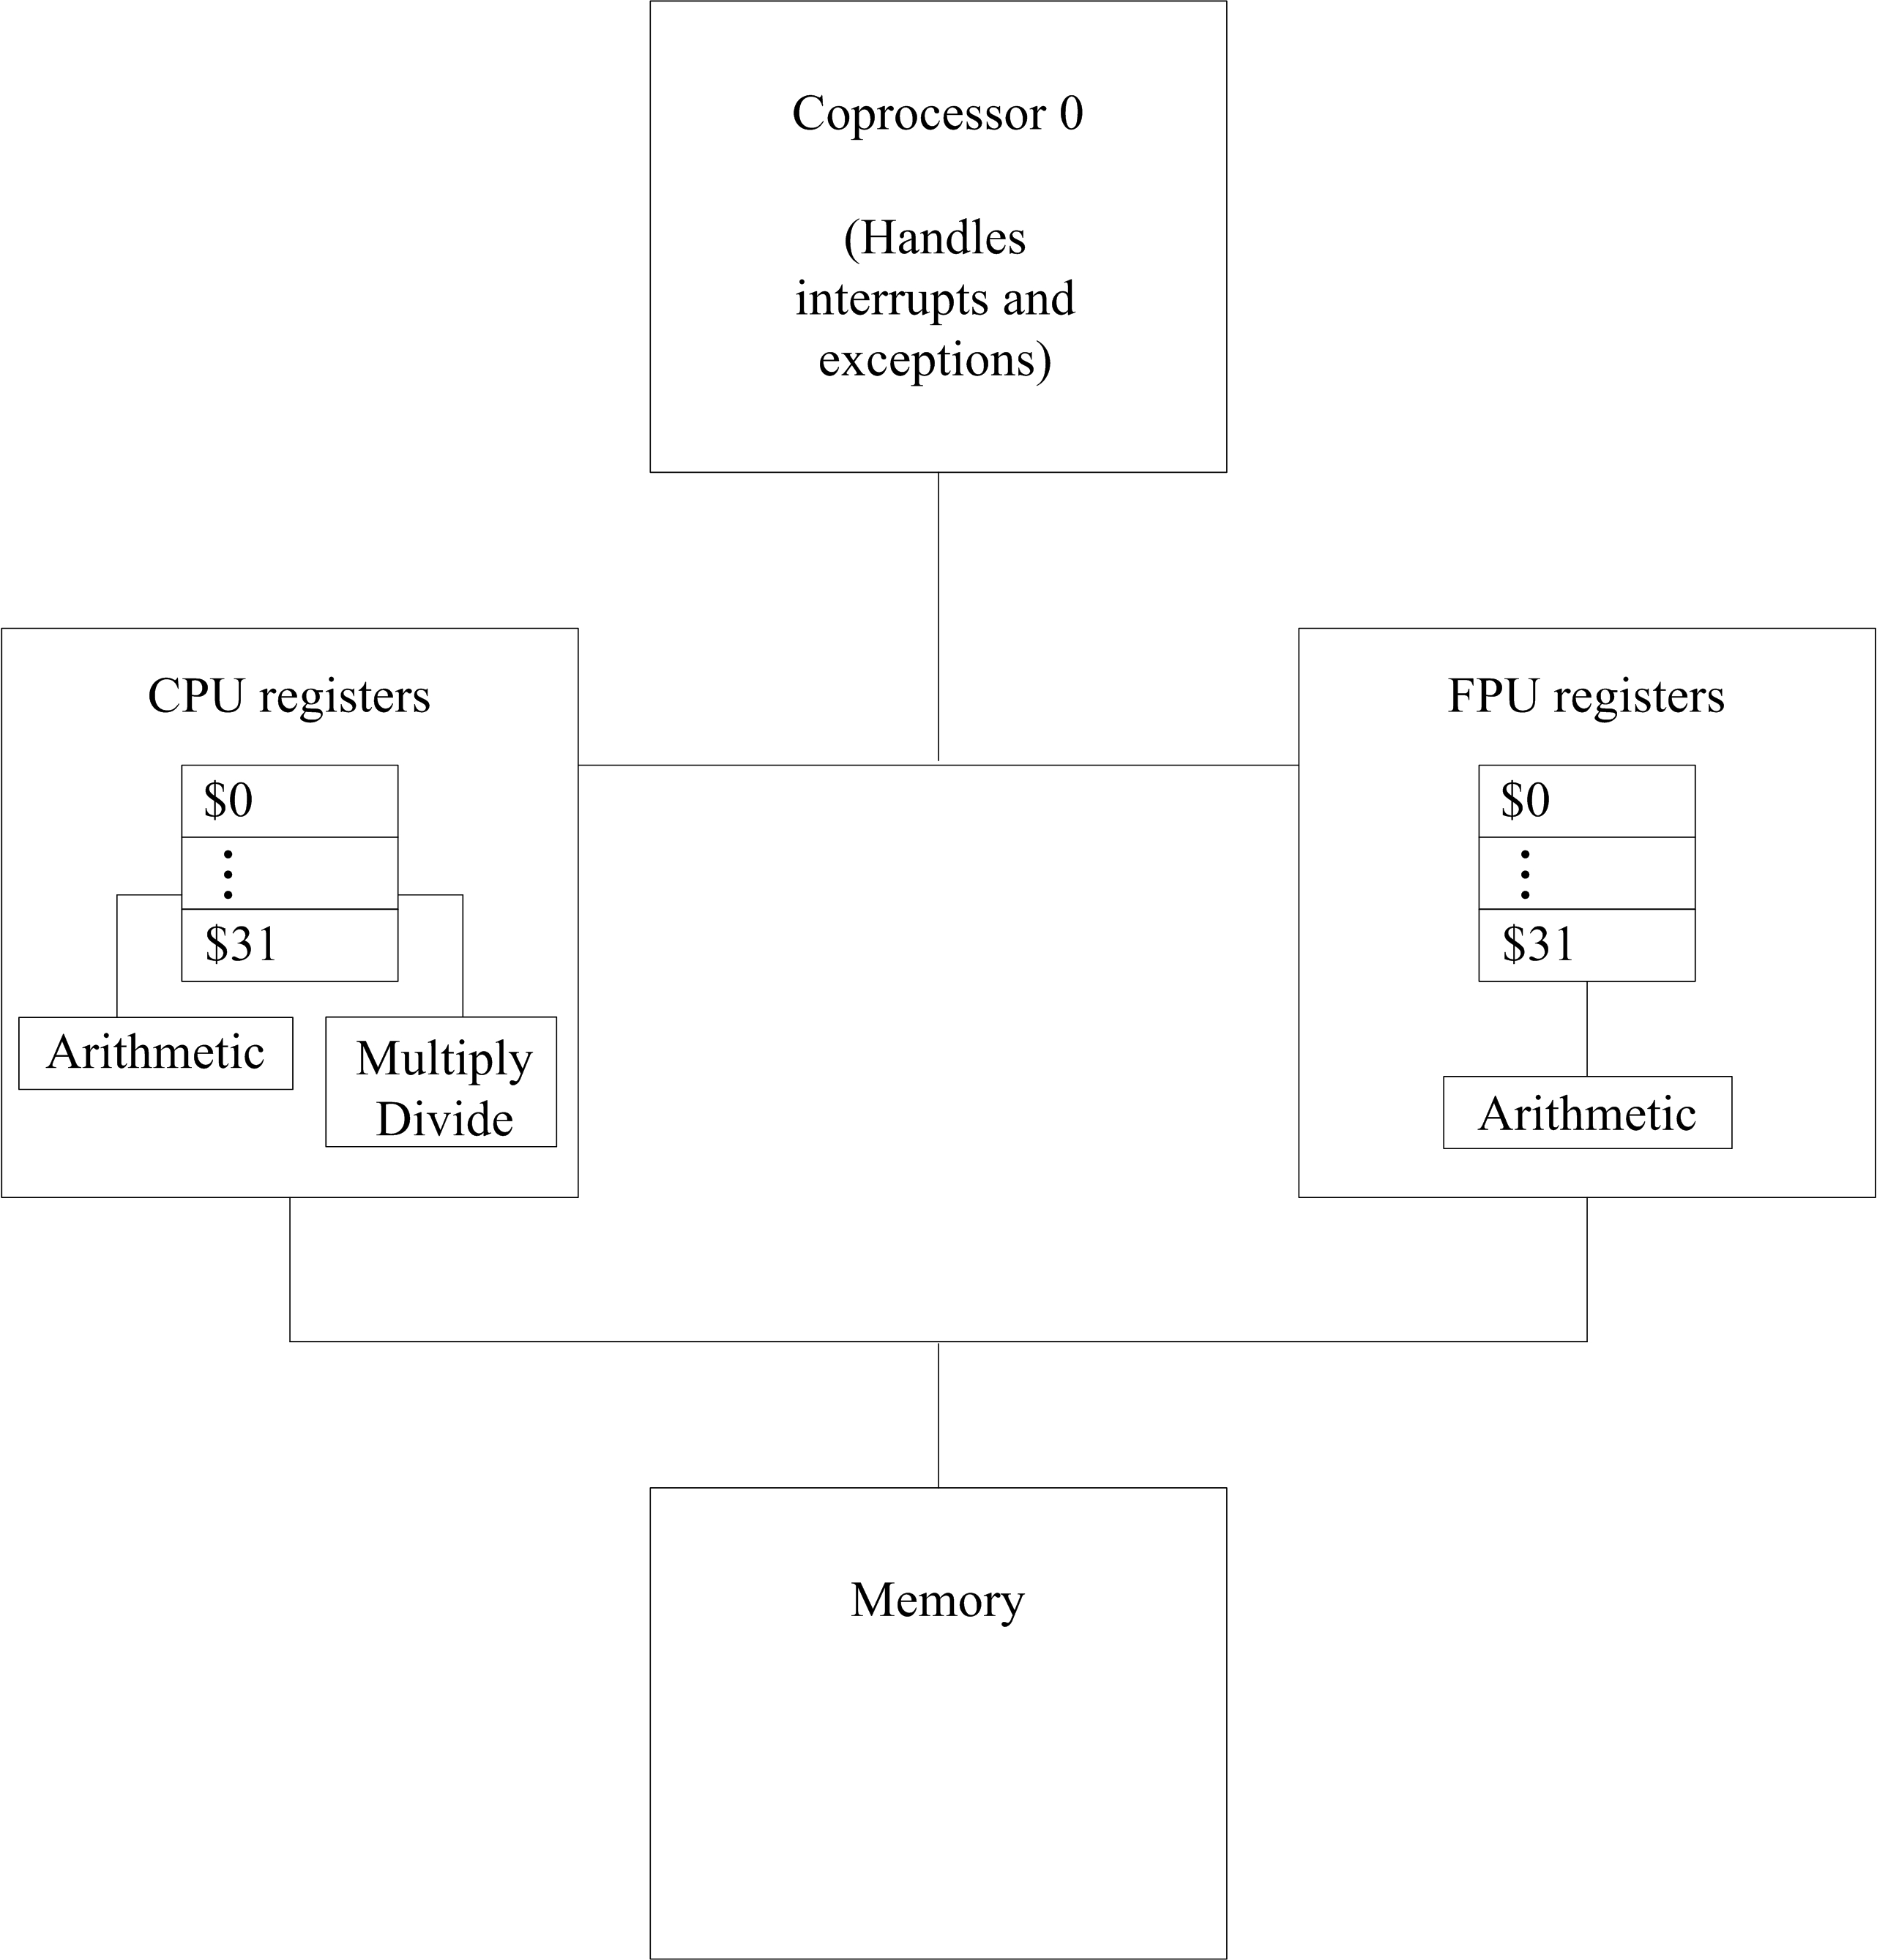
\includegraphics[scale=0.6]{{figures/figure06.02}.jpg}}
\end{center}
\end{frame}

\begin{frame}[fragile]
\pause

Memory organization, by convention divided into four segments, is shown below
\begin{center}
\visible<2->{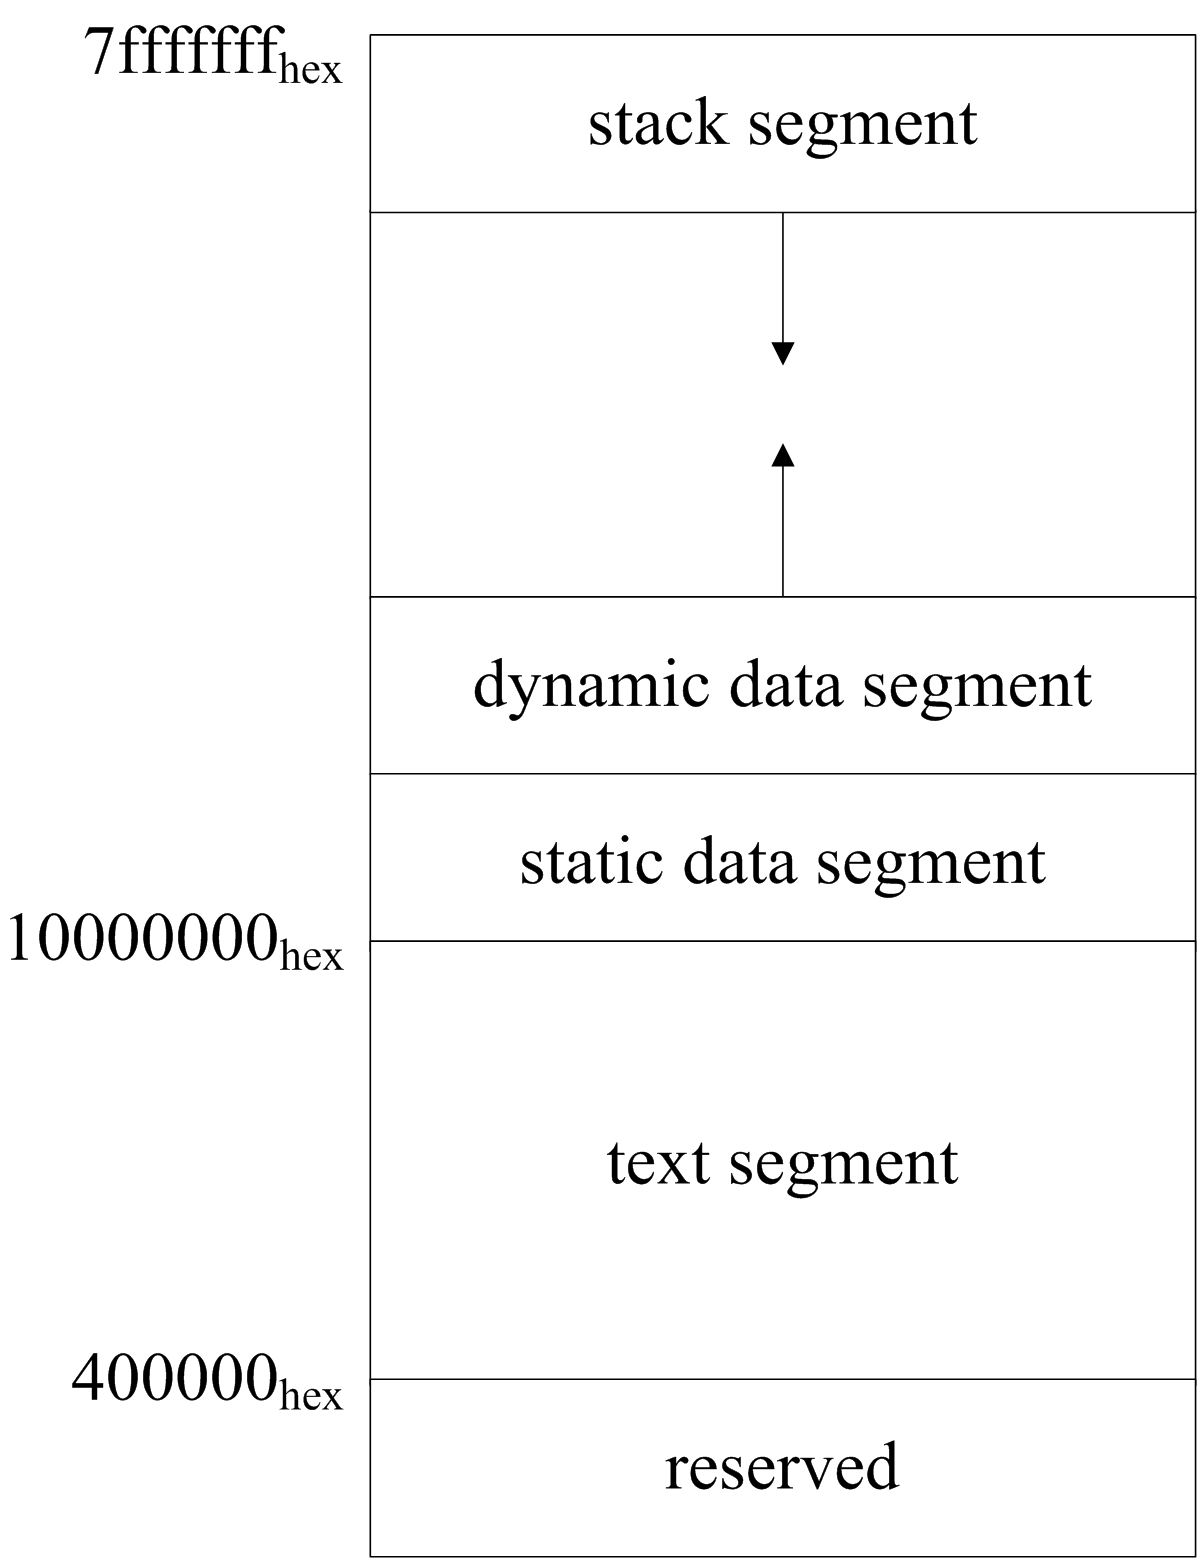
\includegraphics[scale=0.5]{{figures/figure06.03}.jpg}}
\end{center}

\begin{itemize}
\item Text segment - The program's instructions go here
\item Static data segment - Static data, which exist for the duration of the program, go here
\item Dynamic data segment (aka heap) - This is where objects and arrays are dynamically
allocated during execution of the program
\item Like the stack for the JVM, every time a routine is called, a new stack frame is pushed onto the stack; every time a return is executed, a frame is popped off
\end{itemize}
\end{frame}

\begin{frame}[fragile]
\pause

Many of the thirty two (0 -- 31) 32-bit general-purpose registers, by convention are designated for special uses, and have alternative names
\begin{itemize}
\item \$zero (0) always holds the constant 0
\item \$at (1)  is reserved for use by the assembler
\item \$v0 and \$v1 (2 and 3) are used for expression evaluation and as the results of a function
\item \$a0 -- \$a3 (4 -- 7) are used for passing the first four arguments to routines; any additional
arguments are passed on the stack
\item \$t0 -- \$t7 (8 -- 15) are meant to hold temporary values that need not be preserved across
routine calls; if they must be preserved, it is up to the caller to save them
\item \$s0 -- \$s7 (16 -- 23) are meant to hold values that must be preserved across routine calls; it is up to the callee to save these registers
\item \$t8 and \$t9 (24 and 25) are caller-saved temporaries
\item \$k0 and \$k1 (26 and 27) are reserved for use by the operating system kernel
\item \$gp (28) is a global pointer to the middle of a 64K block of memory in the static data segment
\item \$sp (29) is the stack pointer, pointing to the last location on the stack
\item \$fp (30) is the stack frame pointer, pointing to the latest frame on the stack
\item \$ra (31) is the return address register, holding the address to which execution should continue upon return from the latest routine
\end{itemize}
\end{frame}

\begin{frame}[fragile]
\pause

SPIM assumes we follow a particular protocol in implementing routine calls, when one
routine (the caller) invokes another routine (the callee)

\pause
\bigskip

Most bookkeeping for routine invocation is recorded in a stack frame on the run-time stack segment, as is done in the JVM; but here we must also deal with registers

\pause
\bigskip

The stack frame for an invoked routine is shown below
\begin{center}
\visible<4->{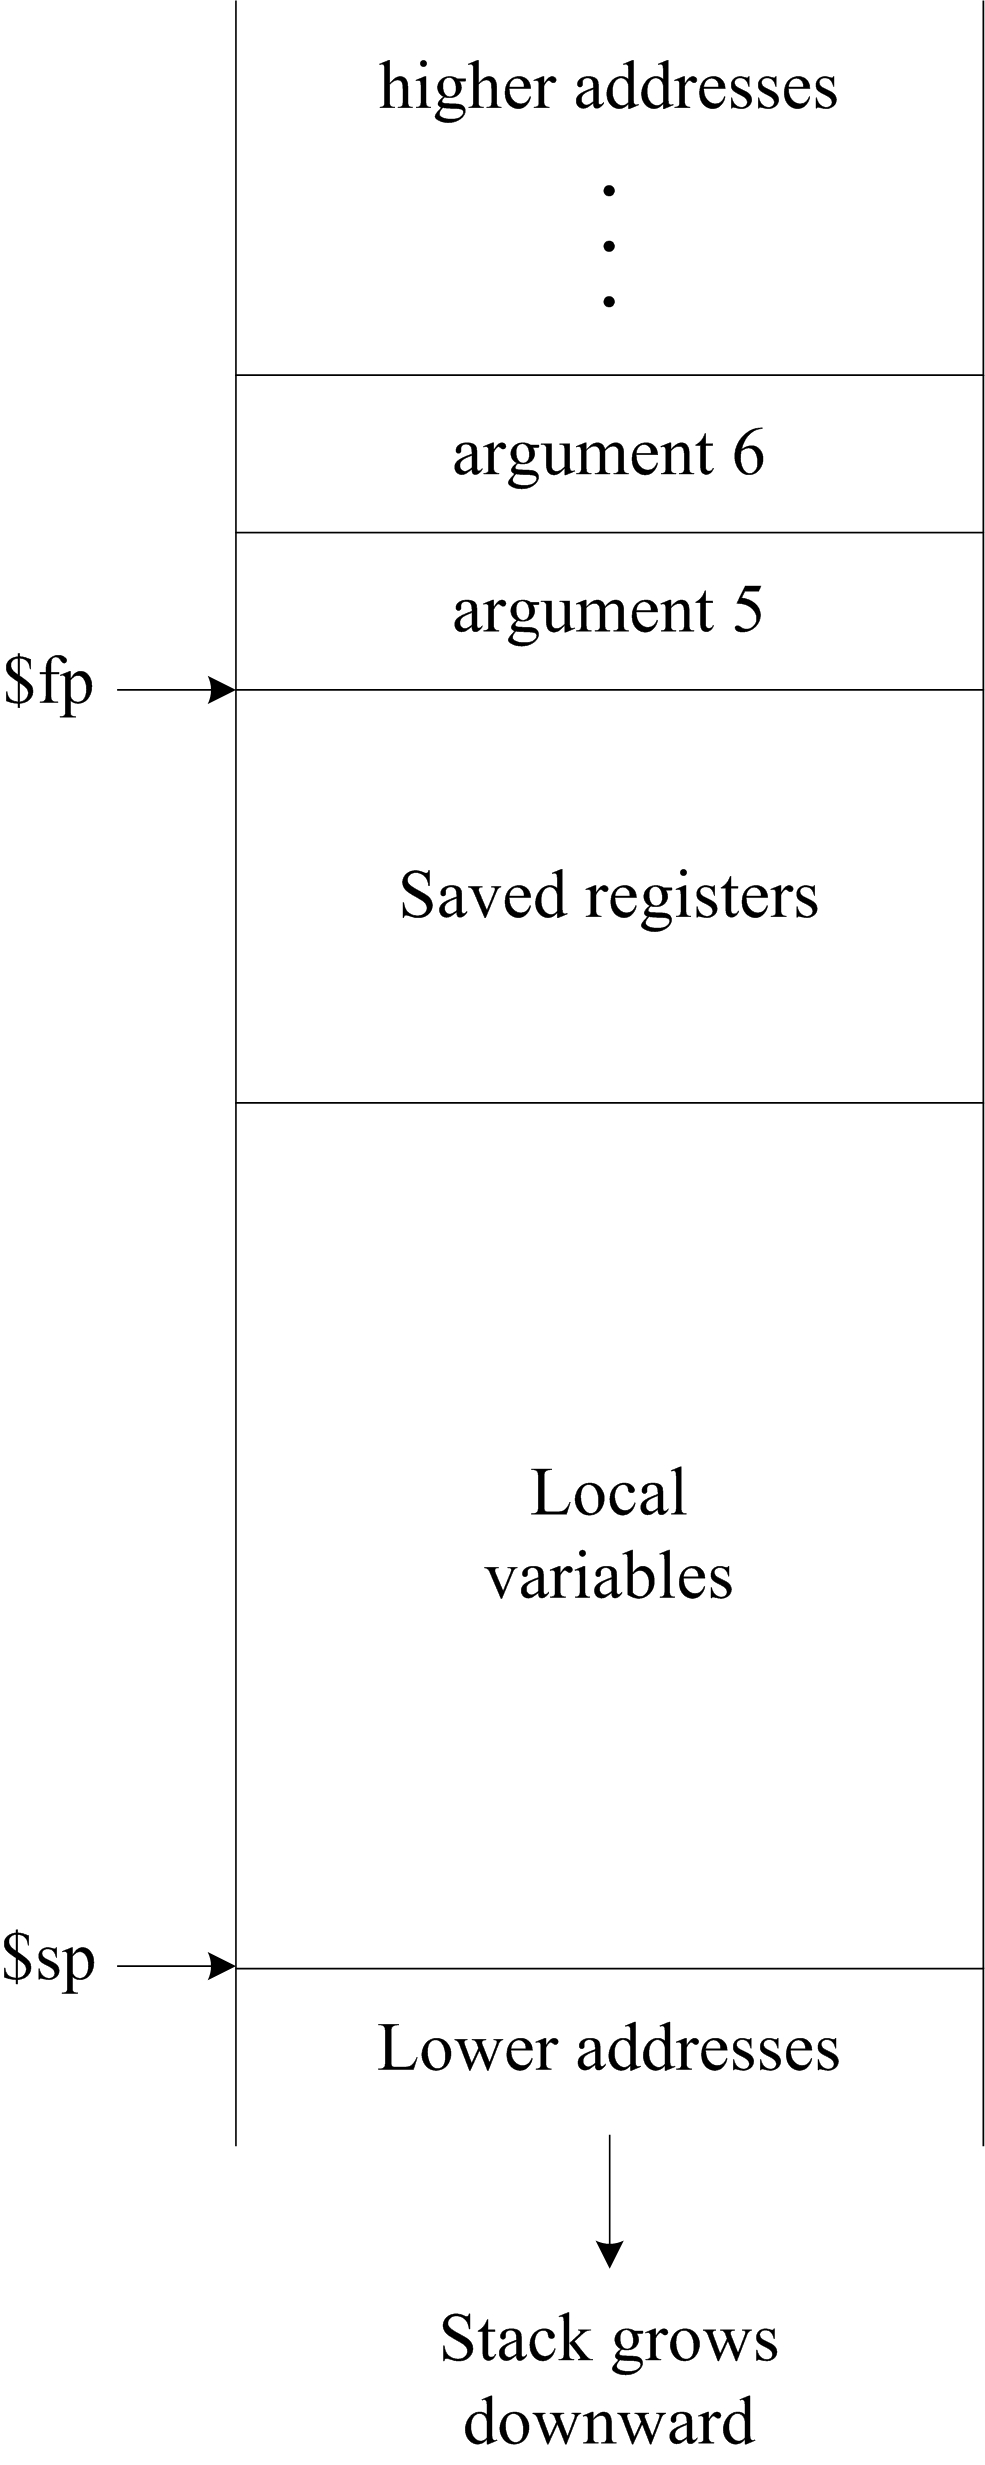
\includegraphics[scale=0.4]{{figures/figure06.04}.jpg}}
\end{center}

\pause
\bigskip

SPIM provides a set of system calls for accessing simple input and output functions
\end{frame}

\section{Our Translator}
\begin{frame}[fragile]
\pause

\end{frame}
\end{document}
